%!!!!!!!!!!!!!!!!!!!!!!!!!!!!!!!!!!!!!!!!!!!!!!!!!!!!!!!!!!!!!!!!!!!!!!!!!!!!!!
%!NOTE: This example file has been prepared according to the University of
%!      Hawaii Style & Policy Manual for Theses and Dissertations dated
%!      "Revised September 2010". If you have one with a later date, you may
%!      need to make revisions to this document as well. In any event, making
%!      sure your thesis complies with Graduate Education guidelines is
%!      ultimately your responsibility. Caveat LaTeXtor. :)
%!!!!!!!!!!!!!!!!!!!!!!!!!!!!!!!!!!!!!!!!!!!!!!!!!!!!!!!!!!!!!!!!!!!!!!!!!!!!!!

%% The options are (you can only choose one from each group):
%%
%% 10pt, 11pt, 12pt: chooses the point size for the document. "11pt" is the
%%                   default.
%%
%% oneside, twoside: whether you want your document onesided or twosided. Note
%%                   that twosided is not guaranteed to work, and style
%%                   guidelines prohibit double sided printouts on final
%%                   copy. "oneside" is the default.
%%
%% draft, final: when printing drafts you can save a lot of paper by using the
%%               "draft" option. It switches to single spacing, displays overful
%%               hboxes with a black box, prints a version number on title page 
%%               and omits signature page. Of course for the final copy make
%%               sure to use the "final" option! "final" is the default.
%%
%% thesis, dissertation: switches between the style for a master's thesis and a 
%%                       Ph.D. dissertation. The differences are fairly minor
%%                       and limited to the front matter. "thesis" is the
%%                       default.
%%
%% actual, proposal: switches between actual document and proposal mode. In
%%                   proposal mode: the title page is simplified and the
%%                   version number is always printed.
%%
%%% Load the new uhthesis document class
\documentclass[12pt]{article}

\usepackage[table,xcdraw]{xcolor}
\usepackage{setspace}
\usepackage{paralist}
%\usepackage{amsmath}
\usepackage{bm}
%\usepackage{subfigure}
\usepackage{cite}
\usepackage{multirow}
\usepackage{todonotes}
\usepackage{umoline}
\usepackage{xspace}
\usepackage{soul}
%\usepackage{gensymb}
\usepackage[euler]{textgreek}
\usepackage{array}
\usepackage{tabu}
\usepackage{tabularx}
\usepackage{subcaption}
\usepackage{amsmath}
%\usepackage{table}
%\usepackage{xcolor}
%\usepackage{xcdraw}

%%% Custom Macros %%%
\newcommand\tab[1][1cm]{\hspace*{#1}}
\newcommand{\LL}[2][inline]{\todo[color=red!50,#1]{\sf \textbf{LL:} #2}\xspace}
\newcommand{\HC}[2][inline]{\todo[color=blue!50,#1]{\sf \textbf{HC:} #2}\xspace}
\newcommand{\gridsize}{\texttt{GRID\_SIZE\xspace}}
\newcommand{\celsius}{$^\circ$C\xspace}
\newcommand{\hotspot}{Hotspot\xspace}
\newcommand{\crosstalk}{crosstalk\xspace}
\newcommand{\Crosstalk}{Crosstalk\xspace}
%\newcommand{\alpha}{\textalpha }
%%% Load some useful packages:
%% New LaTeX2e graphics support
\usepackage{graphicx}
%% Package to linebreak URLs in a sane manner.
\usepackage{url}

\usepackage{paralist}

\usepackage{listings}
\lstset{frame=tb,
  language=Python,
  aboveskip=3mm,
  belowskip=3mm,
  showstringspaces=false,
  columns=flexible,
  basicstyle={\small\ttfamily},
  numbers=left,
  numberstyle=\tiny\color{black},
  keywordstyle=\color{blue},
  commentstyle=\color{dkgreen},
  stringstyle=\color{red},
  breaklines=true,
  breakatwhitespace=true,
  tabsize=3
}
\usepackage[T1]{fontenc}
\usepackage{titling}
\setlength{\droptitle}{-1em}
\title{ICS674 Mini Project}

\author{Lambert Leong}


\begin{document}

\textbf{ICS674 Mini Project}
\\    Lambert Leong

%\maketitle

\section{Search Space}

\begin{lstlisting}[caption = {Search space is all letter characters, upper and lower case }]
self.string = ''.join(random.choice(string.letters) for _ in xrange(length))
\end{lstlisting}

\section{Variation Operator}

\subsection{CrossOver}

\begin{lstlisting}[caption = { }]
def crossover(individuals):
        offspring = []
        for _ in xrange((population - len(individuals))/2):
                parent1 = random.choice(individuals)
                parent2 = random.choice(individuals)
                child1 = Individual(in_str_len)
                child2 = Individual(in_str_len)
                split = random.randint(0, in_str_len)
                child1.string = parent1.string[0:split] + parent2.string[split:in_str_len]
                child2.string = parent2.string[0:split] + parent1.string[split:in_str_len]
                offspring.append(child1)
                offspring.append(child2)
        individuals.extend(offspring)
        return individuals
\end{lstlisting}

\subsection{Mutation}

\begin{lstlisting}[caption = {}]
def mutation(individuals):
        for individual in individuals:
                for i, param in enumerate(individual.string):
                        if random.uniform(0.0, 1.0) <= 0.05:
                                individual.string = individual.string[0:i] + random.choice(string.letters) + individual.string[i+1:in_str_len]
        return individuals
\end{lstlisting}


\section{Selection Operator}

\begin{lstlisting}[caption = {}]
def selection(individuals):
        individuals = sorted(individuals, key=lambda individual: individual.fitness, reverse=True)
        max_fit.append(max(individuals, key=lambda individual: individual.fitness).fitness)
        min_fit.append(min(individuals, key=lambda individual: individual.fitness).fitness)
        avg_fit.append(float(sum(i.fitness for i in individuals)//len(individuals)))
        individuals = individuals[:int(0.2*len(individuals))]
        return individuals
\end{lstlisting}

\section{Termination Criterion}

\begin{lstlisting}[caption={}]
 for generation in xrange(generations):
                generation_list.append(generation)
                individuals = fitness(individuals)
                individuals = selection(individuals)
                individuals = crossover(individuals)
                individuals = mutation(individuals)
                if any(individual.fitness >= 100 for individual in individuals):
                        found = True
                        break
\end{lstlisting}
\section{Objective Fuction}

\begin{figure}[h!]
        \centering
        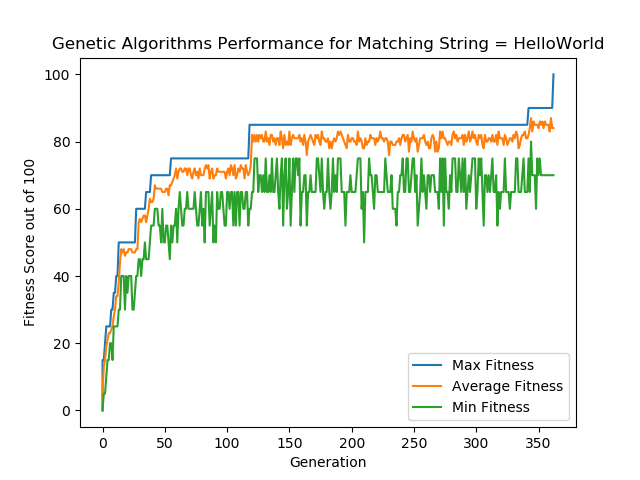
\includegraphics[width=\textwidth]{figures/Figure_3.png}
        \caption{Max, average, and min fitness values of each indvidual string
for each generation}
        \label{fig:fitness}
\end{figure}

\begin{lstlisting}[caption = {Fitness Function}]
def fitness(individuals):
        for individual in individuals:
                total = len(in_str)*2
                score = 0
                for i, letter in enumerate(individual.string):
                                if in_str[i] == letter:
                                        score += 1
                compare_str = in_str
                for a_char in individual.string:
                        for i, in_char in enumerate(compare_str):
                                if a_char == in_char:
                                        score += 1
                                        compare_str = compare_str[:i]+compare_str[i+1:]
                                        break
                individual.fitness = int((float(score)/float(total))*100)                          
        return individuals
\end{lstlisting}
\end{document}
